\documentclass[a4paper,11pt,titlepage]{article}
\usepackage[margin=2cm]{geometry}

\usepackage[nodayofweek]{datetime}
\longdate

\usepackage{fancyhdr}
\pagestyle{fancyplain}
\fancyhf{}
\lhead{\fancyplain{}{M.Sc.\ Individual Project Literature Survey}}
\rhead{\fancyplain{}{\today}}
\cfoot{\fancyplain{}{\thepage}}
\usepackage{adjustbox}

\usepackage[english]{babel}
\usepackage[utf8x]{inputenc}
\usepackage{float}

\usepackage{amsmath}
\usepackage{graphicx}
\usepackage{cite}
\usepackage{hyperref}




\title{Browser-based Medical Image Viewer using WebGL \\\Large{--- Report ---}}
\author{David Basalla\\
  \{db913\}@ic.ac.uk\\ \\
  \small{Supervisor: Dr.\ Ben Glocker}\\
  \small{Imperial College London}
}

\begin{document}
\maketitle



\section{Introduction}

Medical imaging is a type of scientific visualisation that deals with analysis, representation and exploration of medical image data. It should aid in diagnosis, treatment planning, support in actual operations, documentation and educational purposes. Medical imaging is primarily based on 3D volume data acquired by scanning devices such as computed tomography and magnetic resonance imaging. The resulting data files are viewed with specific computer software and contain a wealth of data. Users are therefore required to have the appropriate software installed on their local desktop computer. Additionally software developers have to cater for different operating systems. To overcome these issues, the goal of this project is to provide a medical image viewer that runs in any web browser. This web-app will aim to provide the functionality as a desktop solution without being tied to a specific operating system. It furthermore aims to provide an intuitive and complete set of tools for viewing multiple files and allowing for creation, viewing and manipulation of label maps and other methods of annotating these images. The rationale behind this is to facilitate users to conveniently view, edit and annotate medical image files independently of location or type of computer, following the "Software as a Service" paradigm.

\subsection{Motivations}

\subsection{Requirements}


The goal of this project is to build a web browser based Medical Image Viewer. This will be achieved by making use of \textit{WebGL} to display 2D and 3D graphics. In general the project aims to provide similar functionality and user experience as the desktop application \textit{MITK} (discussed earlier). The essential requirements are as follows:

\begin{itemize}
\item The user can load and view a scan file (of type \textit{NIfTI})
\item The user can view a file in 2D and 3D
\item The user can easily navigate through the 2D and 3D viewers, with emphasis on intuitive user experience
\item The web-app provides controls for viewing the scan files at different brightness and contrast levels
\item The user can load and view a labelmap for a given scan file
\item The user can load additional scan or label maps into the viewer and compare them to previously loaded files with a set of intuitive controls
\item Provide different color-lookups (for label-maps, heat maps)
\item Provide sample data to use if user has no files of his own
\end{itemize}

Given enough time, secondary requirements can be implemented, which are considered to be more complicated:

\begin{itemize}
\item The user can paint a custom labelmap for a given scan file with a set of intuitive tools. The primary goal will be that the user can paint areas manually on individual slices. Provided there is enough time, some semi-automatic painting tools will also be implemented that will allow the user to specify regions in the 3D space with automatic selection tools. 
\item The user can save a labelmap to his computer
\item The user can create and save custom annotation maps to label given scans
\item The web app provides a method for sharing  means of sharing data across the internet (similar to the DropBox implementation in SliceDrop)
\item The web app provides image filters that can be applied to a scan or label map
\item The web app provides measuring tools that can be applied to a scan or label map
\item A three dimensional, parameterised model of the scan be viewed in the 3D view
\item The 'cine mode' feature allows for an animation along a specified axis
\end{itemize}





\subsection{Contributions}

The final software represents a comprehensive tool for viewing medical image data as well as adding custom annotations . All of the primary aims as stated above have been met, as well as a couple of secondary requirements (see full feature list in the Implementation Section). It is designed to be used with intuitive control as advised for use by radiologists, mimicking convential controls in other software. Judging by similar software online, the software provides many more features than its competition. It has also been tested to successfully run across several operating systems and web browsers, thereby fulfilling the requirement of being more widely useable independent of computer configuration of the user. The project was built on using the XTK library, which appears to be the most comprehensive library for viewing medical image data to date. However since missing a lot of critical functionality as required by this project, the library had to be extended to provide tools for more dynamic application building.


\section{Background}



\subsection{Medical Imaging}



As mentioned, medical image files are acquired by scanning devices that output data at a given resolution of data points. A typical medical image file contains a stack of individual images. Each image represents a thin slice of the scanned body part and is made up of pixels. For a volume data set the stack of images can be usually subdivided into cross sections along the three Cartesian axes X, Y and Z and together form a 3D Grid. In medical terms, these orthogonal views are called axial, sagittal and coronal. A constant pixel distance along X and Y allows for accurate measuring of distances and areas along a slice. The slice distance is the measurement in space from one slice to the next along its cross section. The three distances in every direction is called the voxel distance. If the pixel distance is equal to the voxel distance, the dataset is called isotropic. However in practice datasets usually exhibit a much smaller pixel distance than slice distance, which is called anisotropic.
Measuring cross-sectional areas and volumes are valuable for example in diagnosis of vascular diseases. The quality of these measurements is highly dependent on the quality of the image data. Typically diagnosis has been performed these slices one at a time, meaning looking at every slice. These views support precise exploration and analysis and it is a legal requirement for radiologists to inspect every slice. However for spatially complex cases a purely slice-based presentation might not be very helpful. In this case 3D visualisation or volume rendering gives a better overview. The two different visualisations can be helpful for different users, such that radiologists would rely more on the 2D Views and physicians who carry out interventions might find benefit from 3D visualisations. Therefore any software that aims to display such medical image data should provide both views.



\subsection{Guidelines for Medical Image Viewer Software}

As defined in 'Visual Computing in Medicine'\cite{book}, a program needs to provide the following functionality in order to be of use when displaying this kind of medical imaging data. 

First, a certain mapping of data to gray values has to occur, called 'windowing'. This is customisable, but the goal is to display an image with meaningful values so that a user can visually perceive the files. Different mappings or lookup tables (LUTs) can be applied to render the same data with different color or level ranges.

Secondly, the user should be able to easily browse through the slices. The axial, sagittal and coronal views should be provided as well as a 3D dimensional view of these slices in either card-based or volume form. All slices should update accordingly as the user browses through them. However in order to examine a view in detail, it should be possible to enlarge a desired view. Displaying all views at the same usually only serves to give an overview. Additionally a feature called 'cine mode' could be provided which is an animation through one of the slice stacks. This could aid in understanding the spatial relationship of the slices.



Furthermore, the software should provide means to take measurements of the image data, such as distance, area or volume measurements. In this case it is helpful to specify a region of interest (ROI) that can be focused on. Also intensity distribution can be measured to give indications of severity of disease in certain cases (such as osteoporosis)\cite{book}.

For advanced tools, the book suggests providing segmentation tools for identification and marking of certain structures. These tools could be manual so that the user has to paint a region for each slice, or semi-automatic where algorithms select regions following specific rules given by the user, such as threshold-based segmentation or region growing. The resulting segmentation (or label maps) should be overlaid on top of the scan data in a clear manner.

It is also suggested to have tools for annotating files with information. Examples would be creating a region around a specific organ or an arrow pointing to a particular area of interest.
On the topic of user interaction, the book points out that the most frequently used should be carried out with the mouse. Specifically, browsing through slices could be done by scrolling wheel, right-clicking and moving the mouse affect the windowing, ie contrast and brightness. Zooming and panning should also be implemented in similar fashion. These kind of direct mouse controls are preferable to having to adjust specific sliders, although these may be included for visual feedback.

Additional functionality should be added for pressing down the Alt or Shift key and using the mouse.
With regards to 3D rendering of the data, different modes are mentioned. Multiplanar Reformatting (MPR) is a way to creating an arbitrary slicing with an orientation that does not follow the cartesian axes. Maximum Intensity Projection (MIP) is a frequently technique which casts out rays from the viewing plane and highlights voxels with the maximum intensity, mostly used for diagnosis of vascular structures. Surface Shaded Display (SSD) is another visualisation technique that renders the data as 3D shaded surfaces based on a  given threshold. This is achieved by connecting adjacent voxels as polygons. Some simple lighting is applied for shading so depth relations are more recognisable. Finally Volume Rendering produces a semi-transparent rendering of the data voxels where individual voxels' brightness determine their opacity. This is often referred to as direct volume rendering (DVR) as opposed to indirect volume rendering of SSD.

\subsection{NIfTI File Format}

After consulting with the project supervisor, it is deemed sufficient to support the \textit{NIfTI} for format for medical image data. \textit{NIfTI} supports the multi-dimensional format of medical image data as described in the previous section. The format is adapted from the widely used \textit{ANALYZE 7.5} file format. The \textit{ANALYZE 7.5} file format has been widely used in the functional neuroimaging field. The files can be used to store voxel-based volumes. An \textit{ANALYZE 7.5} data item consists of a file with the actual data in a binary format (with the filename extension .img) and another header file (header with filename extension .hdr) with information about the data such as voxel size and number of voxel in each dimension. Among other improvements, the \textit{NIfTI} format allows for storing the two files in one file (with the filename extension .nii), which is an obvious advantage for file management.
In the \textit{NIfTI} format, the first three dimensions are reserved to define the three cartesian spatial dimensions (X, Y, Z). The fourth dimension is reserved to define the time points. The remaining dimensions, from fifth to seventh, are for other uses. 

\subsection{Desktop Applications}

There exists a variety of desktop software to date that allow viewing of medical image data. For this project, a selection of programs have been tested and analysed for functionality.

\subsubsection{MITK 3M3}
Firstly, \textit{MITK 3M3} by Mint Medical and German Cancer Research Center allows for easy viewing of a variety of medical image file formats. The layout of the views is customisable and by default shows the X, Y, Z dimension and a 3D view of all 3 dimensions together. (picture) There is a universal range slider that affects all images at once. Labelmaps (called Segmentations) can be added to a scan file, as sub layers and a range of paint tools are provided to colour in regions of the scan. An arbitrary number of layers can be created and saved out as separate files. 
Furthermore it can create a 3D volume renderings, applying image filters and supplies measuring tools. In general it is a well rounded product with intuitive controls so will serve as a good benchmark test for the final product.

\subsubsection{Imview}
\textit{Imview} is a medical image viewer created by Dr. Ben Glocker, which also allows the user to load scan files and inspect the individual slices of each axis. The user can perform flip transformations and apply different colour look-ups to the image, such as Colormap Jet which looks like a heat map. It also provides the option of displaying an information overlay with stats about the image. It would be beneficial if the web-app has similar options as they provide useful data for the user.

\subsubsection{BrainSuite}

Test about BrainSuite... features...


\subsubsection{3DSlicer}
\textit{3DSlicer} is a free open source software that provides a modular platform for image analysis and visualization. Of all the packages, this tool seems to be the most feature rich, which is not surprising as it is funded by a number of American organisations such as  the National Alliance for Medical Image Computing, Neuroimage Analysis Center and others. Although it features a wide variety of tools, the focus will be on the ones relevant to this project. \textit{3DSlicer} allows for loading of different files of different formats. It provides options to composite different slices on top of each other for comparison. It supports hardware accelerated volumetric rendering of medical image data. It is widely customisable with global settings. Layouts are also customisable. It has an extensive set of tools for manual and automatic image segmentation. It has an in-built feature to download sample data, which would be a useful inclusion for the web app project. Another powerful feature is that \textit{3DSlicer} allows the addition of new functionality and provides a number of generic features not available in competing tools. All in all, \textit{3DSlicer} appears like a well designed, user-friendly program that has an overwhelming amount of functionality. It will be another good benchmark and inspiration for this project.

\subsubsection{MIview}
\textit{MIView} was programmed by Greg Book, is open source and provides much the same functionality as \textit{MITK}. \textit{MIView} is an \textit{OpenGL} based medical image viewer which aims to support a wide range of medical imaging files such as \textit{NIfTI}, and raster images. The main goal of \textit{MIView} is to provide a platform to load any type of medical image and be able to view and manipulate the image. Volume rendering is also supported. Control-wise, support for mouse-wheel scrolling seems erratic, which makes navigation through the slices more cumbersome. Also the buttons tend to be quite small which also does not improve the user experience. It does not appear to support the loading of multiple files together. A number of predefined color look-up tables are provided.

\subsubsection{Photoshop}
Looking further afield to some graphical editing software programs, some interesting functionality can be discovered. Adobe's \textit{Photoshop} is well known software for creating and manipulating 2D imagery. When editing an image, the user works with a document. The user can add as many layers as required and edit each layer individually. The layers are composited to form the whole picture. Each layer's opacity and compositing/blending mode can be specified. This could be a worth while to emulate for comparing different medical image files in the web app.



\subsubsection{Nuke}
The Foundry's \textit{Nuke} is a compositing package which is used in the Visual Effects Industry to edit and composite 2D images with each other. It is used among others at high profile Visual Effects companies such as Industrial Light and Magic and Weta Digital\cite{nuke1} \cite{nuke2}). The interface differs from \textit{Photoshop} in that it provides the user with a workplace where any number of nodes can be created. When selecting any node, a graphical display will appear. These nodes can be linked together and do anything from loading a specific image file, transforming the whole node tree or applying an image filter such a film grain. The power of this approach is the modular nature of a tree. Any node can be taken out and reinserted at another place into the tree, thereby changing the final image. Additionally, for comparing different images, by default the software supplies two image buffers which the user can fill with any image of his choice (including of course the result from any node tree in his workspace). Once both buffers are filled, the user can easily toggle between the two images, blend between them by setting the opacity and even use a slider to reveal just a portion of either image. So while \textit{Nuke}'s node-based approach may be overkill for this project, \textit{Nuke}'s image blending seems quite desirable for this project as it would give the user a variety of ways in which he can compare multiple images. 


\subsection{Web Applications for Medical Image Viewing}


\subsubsection{Web Framework XTK}

As suggested in the project specification, the goal of this project is to use the \textit{X Toolkit}(\textit{XTK}), a \textit{JavaScript}-based framework for visualizing and interacting with medical imaging data using \textit{WebGL}. It was developed and maintained by Haehn et al of the Fetal-Neonatal Neuroimaging and Developmental Science Center at Childrens Hospital Boston, Harvard Medical School, US (\cite{xtk}). \textit{XTK} provides an API to load medical images, based on \textit{WebGL} technology for displaying 3D graphics and the \textit{HTML5} canvas elements to display 2D components. It hides a lot of the low-level elements of \textit{WebGL} and is designed to load and configure medical image data files of various types (including \textit{NIfTI}). The library is well documented and comes with several tutorials as well as a number of example applications, which will be discussed in the next section. It appears to follow closely the suggestions laid out in section 2.1 (Medical Imaging) in that it provides means to display 2D and 3D slice visualisations (Surface Shaded Display and Volume Rendering are supported), with simple mouse-based controls. It allows for loading of label (segmentation) maps which can overlaid on top of the image data files. It also features color tables (LUTs) to display the data.

The \textit{XTK} library also provides a module for creating User Interface (UI), that can be overlaid on top of the image viewers, with easy controls to connect the image content with the UI controls.
The popular forum for coding questions Stackoverflow hosts about 100 questions regarding \textit{XTK} to date, and occasionally the \textit{XTK} developers offer up answers.




\subsubsection{SliceDrop}
The \textit{XTK} library also provides links to example applications. One of these is \textit{SliceDrop}\cite{slicedrop} which has written by the \textit{XTK} developers and appears to be a testing bed for many of \textit{XTK}'s features as it is often referred to on the \textit{XTK} Stackoverflow forums. It provides part of the desired functionality and shows off the possibilities provided by \textit{XTK}, but also outlines some of its short comings. Like the desktop software \textit{MITK}, the user can load a file and view it in the standard 4 views, split into 3D and 2D windows. The layout of these views is somewhat customisable, although not to the extent of the \textit{MITK}. The user can interact with the images by scrolling the mouse wheel, which changes the index of the current slice. An interesting feature which has been added lately is the incorporation of popular file sharing site \textit{DropBox} to allow users to share files more easily across the internet.

There appear to be some bugs in \textit{SliceDrop}. When loading \textit{NRRD} files, as the image is offset and not centered. The image brightness controls seem not calibrated correctly, as with little mouse interaction, the brightness will clamp to white or black and can not be reset other than restarting the program (refreshing the page for web-apps). Furthermore the app does not allow to load custom labelmaps. Also the viewers provide some functionality which is not clearly communicated to the user, such as holding the 'shift' button and move the mouse will adjust the slice index of the other viewers. In general \textit{SliceDrop} has less than the minimum functionality required for this project, but shows the potential of the \textit{XTK} library. 


\subsubsection{Brainbook}
\textit{Brainbook}\cite{brainbook} is a web-app which builds on and extends the features of \textit{SliceDrop} by adding painting tools. It allows the user to paint onto a given file with a standard brush a number of auto selection tools which will fill out a region in 2D or 3D space. The web app offers to save the file, but at time of writing this feature was not working correctly. Since heavily based on \textit{SliceDrop}, it features similar advantages and disadvantages, but provides the painting functionality that is desirable for this project. Therefore it should be of benefit to study this implementation.

\subsubsection{DWV - DICOM Web Viewer}
This viewer does not provide much functionality other than scrolling through one stack of slices. The user interface is sparse and does not give sufficient feedback to the use of what is currently happening. It uses the \textit{HTML5} Canvas element to display the file contents.



\subsubsection{Papaya}
Papaya\cite{papaya} is a \textit{JavaScript}-based medical image viewer with limited functionality. It has a clean uncluttered design, is easy to use and gives good visual feedback to the user. It successfully adheres to the user control guidelines outlined in section 2.1. It only displays 2D views of slices and does not allow any customisation in terms of label maps, windowing or compositing. It also uses the \textit{HTML5} Canvas element to render the 2D data.



\subsubsection{Other}

The website \url{http://www.idoimaging.com} lists a number of other available browser-based viewers.


\subsection{Developing Web Applications}

\subsubsection{Web Browsers}

According to web browser usage statistics for 2014, the 4 most used
browsers are (in descending order) Chrome, Internet Explorer, Firefox
and Safari. Show the graph from that website. Discuss more. Chosing to focus on Chrome primarily. Chrome because of Android?


Talk about operating systems

Talk about screen resolution

Test!

To make things even more difficult, various programming aspects such as CSS and core DOM functionality is supported to varying degrees in the different browsers and versions. The following site aims to provide a comprehensive breakdown of provided features.

http://www.quirksmode.org/

It is anticipated that all the variations will become a source of problems when developing the project.



\subsubsection{Developing websites}

Talk about DOM


Generally, JavaScript code gets downloaded and executed at the user end.


Programming for modern webpages which require more complex behaviour than just displaying information can get quite involved. Generally it takes at least \textit{HTML}, \textit{CSS} and \textit{JavaScript} to create a useful website. It is possible to include the code from each language in the main index.html file, but this is undesirable as it lacks modularity and will be hard to test and debug.



\subsubsection{Web Frameworks for Single Page Apps}

Talk about MVC paradigm. Talk about MVP paradigm.

At the time of writing, \textit{Backbone} seems to be a good choice to manage the complexity and structure of the project. \textit{Backbone} is used to structure client-side applications (those that run in a web browser). It was written by Jeremy Ashkenas and is designed for developing single-page web applications, and for keeping various parts of web applications synchronized. It is based on the model–view–presenter (MVP) application design paradigm, providing Events, Models, Collections and Views. Models represent the information in class-like structures, Collections are lists of Models and Views handle the visual representation on the actual HTML site. Finally Events are used to keep track of state changes across the website elements, models and views. It builds on \textit{jQuery} and \textit{Underscore.js}, both libraries which simplify dealing with \textit{HTML} elements. It also provides inheritance for its models, collections and views.

Regarding the design aspect, it looks like twitter-bootstrap.js supplies a convenient library for creating visually pleasing user interface elements. This will cut down on having to spend time to design custom elements with \textit{CSS} and \textit{JavaScript}. \textit{Bootstrap.js} supplies buttons, drop-down menus and commonly-used icons. Some specific UI control elements are not provided by \textit{Bootstrap.js}, so \textit{jQueryUI} will be used. It enables the creation and customisation of complex elements such as slider elements with multiple slider tabs, which will allow for a better user experience. Also, it's dependent on the \textit{jQuery} library which is already being used for \textit{Backbone}.

As this project will make of several modules, it will be important to manage the dependencies of the modules. For example \textit{Underscore.js} and \textit{jQuery} will need to load before \textit{Backbone.js} is used. \textit{XTK} and twitter-boostrap are additional modules that will have to be loaded. \textit{RequireJs} is a \textit{JavaScript} library that provide the ability to asynchronously load nested dependencies. Traditionally \textit{JavaScript} files or modules are loaded sequentially, where the order matters in case a module depends on another module. Additionally it will be helpful to manage the different HTML templates required for the various elements of the web app. \textit{RequireJs} will make it possible to split up everything into neat modules and templates and facilitate testing of all the components.



\subsection{Interactive Graphics for Web Applications}

In order to create an interactive web browser application that provides graphical feedback, the available tools for creating 2D and 3D graphics in a web browser have to be considered. Generally, in the past web browsers have provided several different methods to display 2D and 3D graphics on screen, and only recently with the introduction of \textit{HTML5} and \textit{WebGL} has a widely-conformed standard emerged.

\subsubsection{HTML5}

\textit{HTML} or HyperText Markup Language is the standard markup language used to create web pages. \textit{HTML5} is the fifth revision of the standard. \textit{HTML5} introduced a number of important features that were designed to facilitate including and handling multimedia and graphical content on the web without the use of proprietary plugins and APIs. One of these new features is the Canvas element, a scriptable graphical display element which is a low level, procedural model that updates a bitmap element. It was originally introduced by Apple \cite{canvas} .

\subsubsection{2D Graphics}

Displaying 2D graphics has long been an integral part of web browsers. Various aspects and methods allow for the generation and manipulation of 2D graphics in a web browser. Aside from simply displaying an image file, there are various other aspects and methods allow for the generation and manipulation of 2D graphics in a web browser

\textit{CSS} is used to alter an element's style property, but this is not really suitable for creating intricate 2D graphics, as it is typically used to style the look of \textit{HTML} elements. There are no custom draw commands.

Scalable Vector Graphics (\textit{SVG}) is like \textit{HTML} for graphics\cite{svg}. It is a markup language for describing all aspects of an image or Web application, from the geometry of shapes, to the styling of text and shapes, to animation, to multimedia presentations including video and audio. It is fully interactive, and includes a scriptable DOM as well as declarative animation (via the SMIL specification). It supports a wide range of visual features such as gradients, opacity, filters, clipping, and masking.
The use of \textit{SVG} allows fully scalable, smooth, reusable graphics, from simple graphics to enhance \textit{HTML} pages, to fully interactive chart and data visualization, to games, to standalone high-quality static images. \textit{SVG} is natively supported by most modern browsers (with plugins to allow its use on all browsers), and is widely available on mobile devices and set-top boxes. All major vector graphics drawing tools import and export \textit{SVG}, and they can also be generated through client-side or server-side scripting languages.

Finally, the Canvas API is a client-side scripting technology to allow for the rich creation or alteration of raster images (bitmaps) . It uses vector-based programmatic methods to create shapes, gradients, and other graphical effects, and because it has no DOM, it can perform very quickly. Dedicated scripters can develop games or even full-featured applications using the Canvas API, alone or integrated into \textit{HTML} or \textit{SVG}. It is supported natively in most modern browsers (with script libraries extending support to all major browsers), and even on some mobile devices.

Before the Canvas API became common place, there were different web browser plug-ins which would display more interactive graphics and videos. Adobe's \textit{FlashPlayer} and JavaApplets were very common for this purpose.
\subsubsection{3D Graphics}

3D Graphics are usually defined by a space in Cartesian coordinates in which reside three-dimensional objects, as well as a camera object through which the scene is viewed with help of a projection matrix. 3D graphics includes lots of maths with matrices and is computationally much more expensive than drawing 2D graphics. Rendering a scene can mean that the image should be refreshed 60 times a second, which poses a challenge for many browsers.

Broadly speaking, the history of 3D Graphics can be divided into the time before and after the standardisation of \textit{WebGL}. Before \textit{WebGL} the standard way to display 3D graphics in a web browser were tied to a browser plug-in that the user would have to download locally to their computer. Adobe's Flashplayer used to be one of the dominant plug-ins. Demonstrating one of the issues with the plug-ins is that they would have to be implemented specifically for each operating system. Furthermore, Apple actually refused to support the format, instead betting on the \textit{HTML5} standard. This shows that there are issues with using browser plug-ins, and a more generalised solution was sought for.

Various other brower-plugins existed or are still around, such as Adobe's \textit{FlashViewer} and \textit{O3D}. \textit{Java Applets} are another alternative, which run on the local machine through the \textit{Java} virtual machine. Microsoft implemented its own plugin \textit{Silverlight}.

With the standardisation of \textit{HTML5}, \textit{WebGL} and the Canvas element became widely used and supported, and helped to reduce the multitude and clutter of browser-plugins. \textit{WebGL} is a \textit{JavaScript} API that exposes a computers GPU to the web browser and allows for displaying of complex three dimensional graphics as seen in comparable desktop applications. Although only initially relased in 2011, \textit{WebGL} is widely supported by most modern browsers (\cite{webGL}), so it's a good time to make use of this for medical visualisation. \textit{WebGL} is based on OpenGL ES 2.0 and uses the \textit{HTML5} canvas element to draw onto and is accessed using Document Object Model interfaces.

Nowadays, most libraries make use of \textit{WebGL} and even libraries that used to require a plug-in (example) have now been ported to use \textit{WebGL}. 











\section{Design and Theory}

Copy From Literature Review
Extend?


\section{Implementation}

\subsection{Implemented Features}

At the end of the project, the software has the following feature list.

\begin{itemize}
\item Display Layer Management

  \begin{itemize}
  \item Creation/Deletion of Display Layers
  \item Loading Medical Image Data File per Display Layer
  \end{itemize}

\item Loading of NII Volume Files (one per Display Layer)	
\item Changing of Brightness
\item Changing Image Threshold
\item Changing indices of NII Volume File
\item Viewing of NII Volume File through 4 bespoke cameras (X, Y, Z and 3D)
\item Custom Layouts of the 4 different cameras
\item Ability to pan/zoom and rotate the NII Volume File through the cameras
  item Ability to traverse by left-click and drag on a 2D-Renderer will update the other 2D Renderers to the current indices
\item Refocus the cameras by pressing 'F'
\item Two buffers to hold different Display Layers
\item Buffer Opacity and Buffer Swiping to compare the two Display Layers
\item Changing the color lookup table for a Display Layer, currently 3 supported Lookups (None, ID's and JET)
\item Toggle for Volumetric Rendering of the Data in 3D Camera View
\item Interactive Annotation Management

  \begin{itemize}
  \item Creation/Deletion of Annotation(s)
  \item Support for multiple Annotations
  \item Customisation of Label, Color and Position of Annotation
  \item Saving out of Annotations as JSON file (via file download)
  \item Loading and Importing of Annotation JSON files
  \item Setting visibility of Annotations
  \end{itemize}

\item Labelmap Management

  \begin{itemize}
  \item Loading of Labelmaps
  \item Changing opacity of Labelmap
  \item Changing color lookup of Labelmap
  \end{itemize}

\end{itemize}


\subsection{Layout and Input Breakdowns}

The main view that the user first sees is split into a 4 different components. The Navigation Bar (in blue colour) contains the links to other sites such as Tutorials, Sample Data and the About webpage. It also contains the Layout Selector buttons where the user can chose a layout for the View Panels. The Display Layer Panel allows for managing of Display Layers, which are synonimous with loaded Volume files. Each Display can load a Volume File. The Levels panel contains various controls for affecting the currently selected Display Layer and its inherent Volume File. Finally the Viewer Panel contains the 4 different Camera View Panels that each Volume is display in. They are the perspective 3D View, and the orthogonal X, Y and Z views.

\begin{figure}[ht!]
\centering
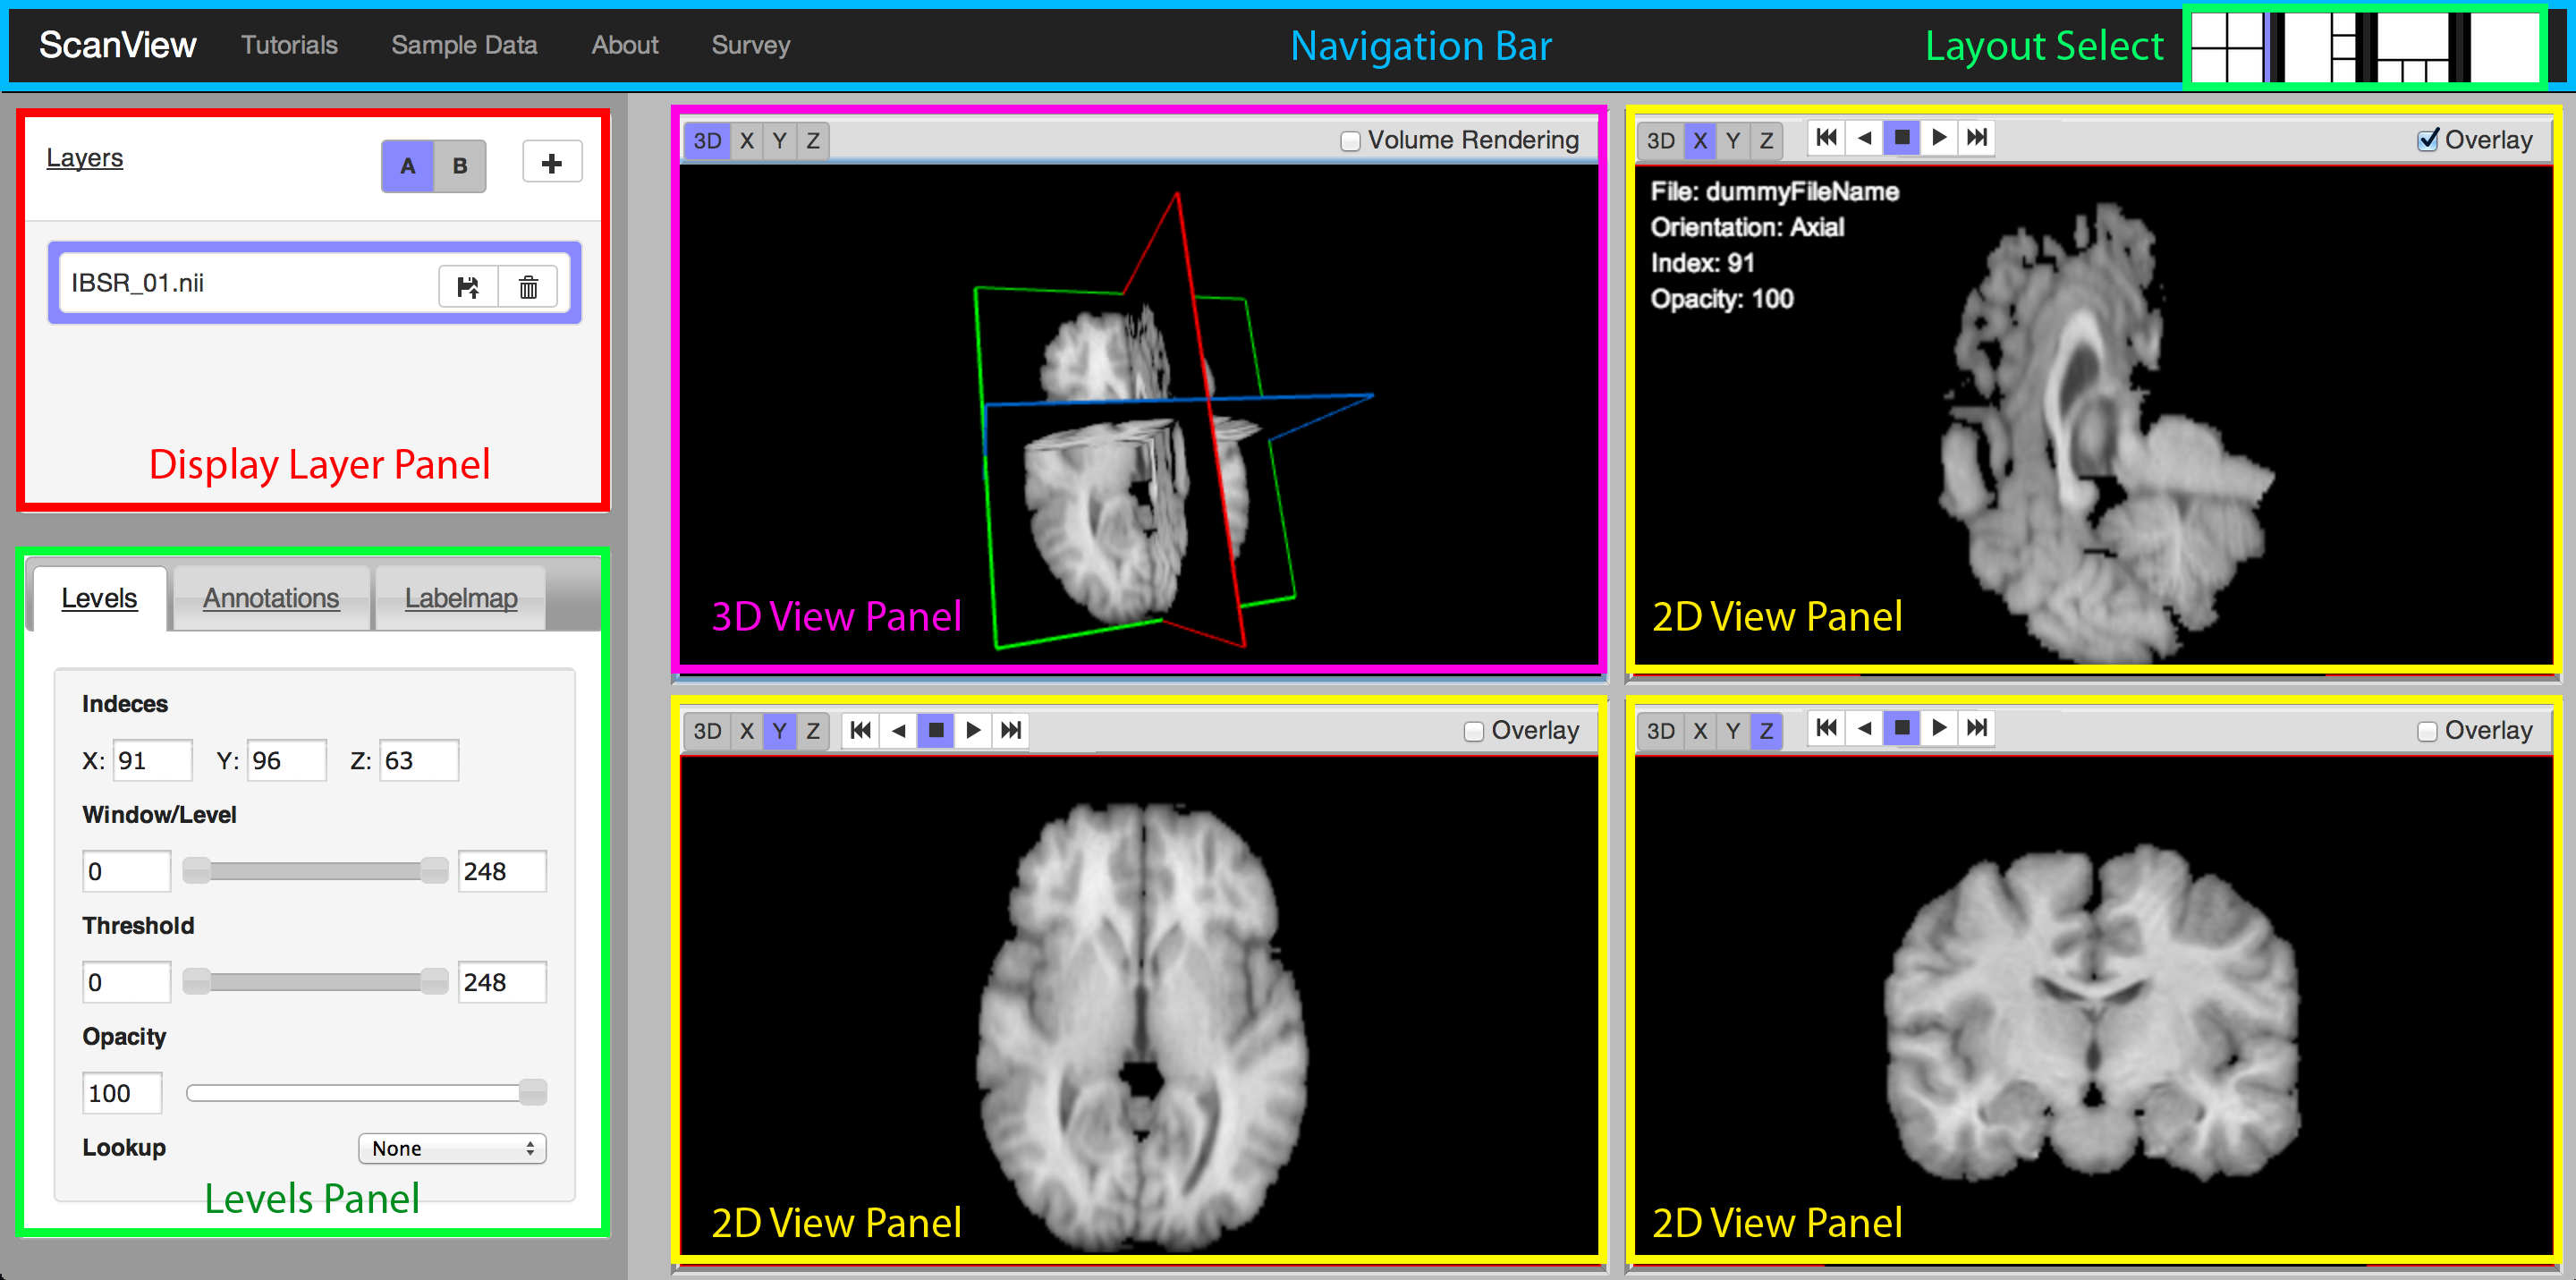
\includegraphics[width=170mm]{graphics/features_01.png}
\caption{General Panel Breakdown}
\label{fig:UIdesign1}
\end{figure}





\begin{figure}[ht!]
\centering
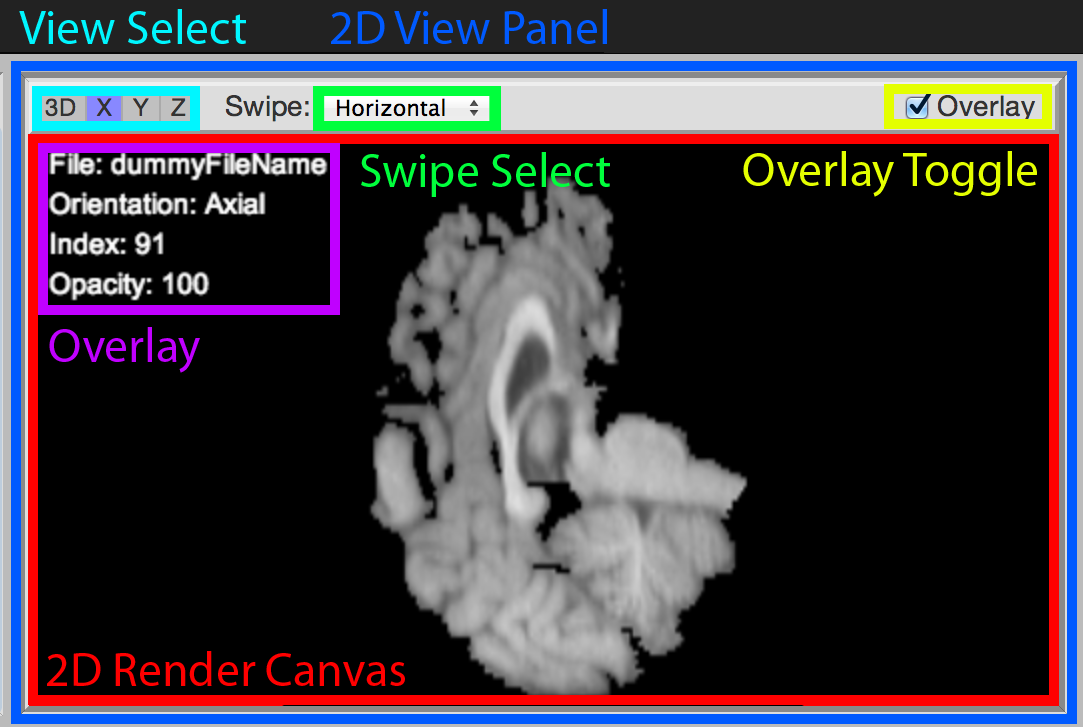
\includegraphics[width=90mm]{graphics/features_02.png}
\caption{2D View Panel Functionality}
\label{fig:UIdesign1}
\end{figure}




\begin{figure}[ht!]
\centering
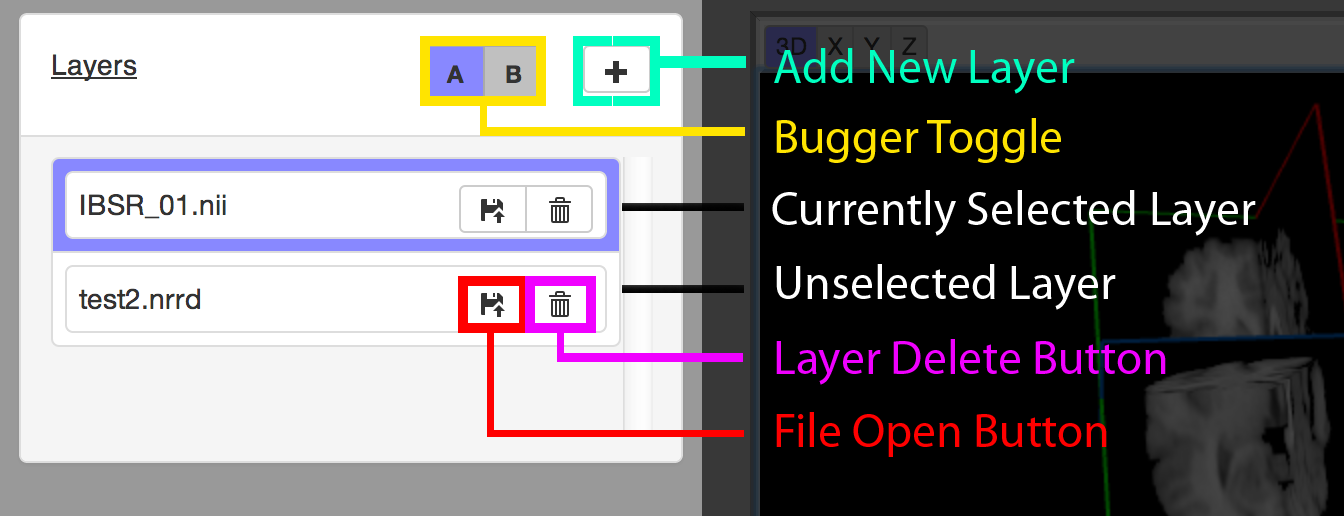
\includegraphics[width=90mm]{graphics/features_03.png}
\caption{Display Layer Panel Functionality}
\label{fig:UIdesign1}
\end{figure}


\begin{figure}[ht!]
\centering
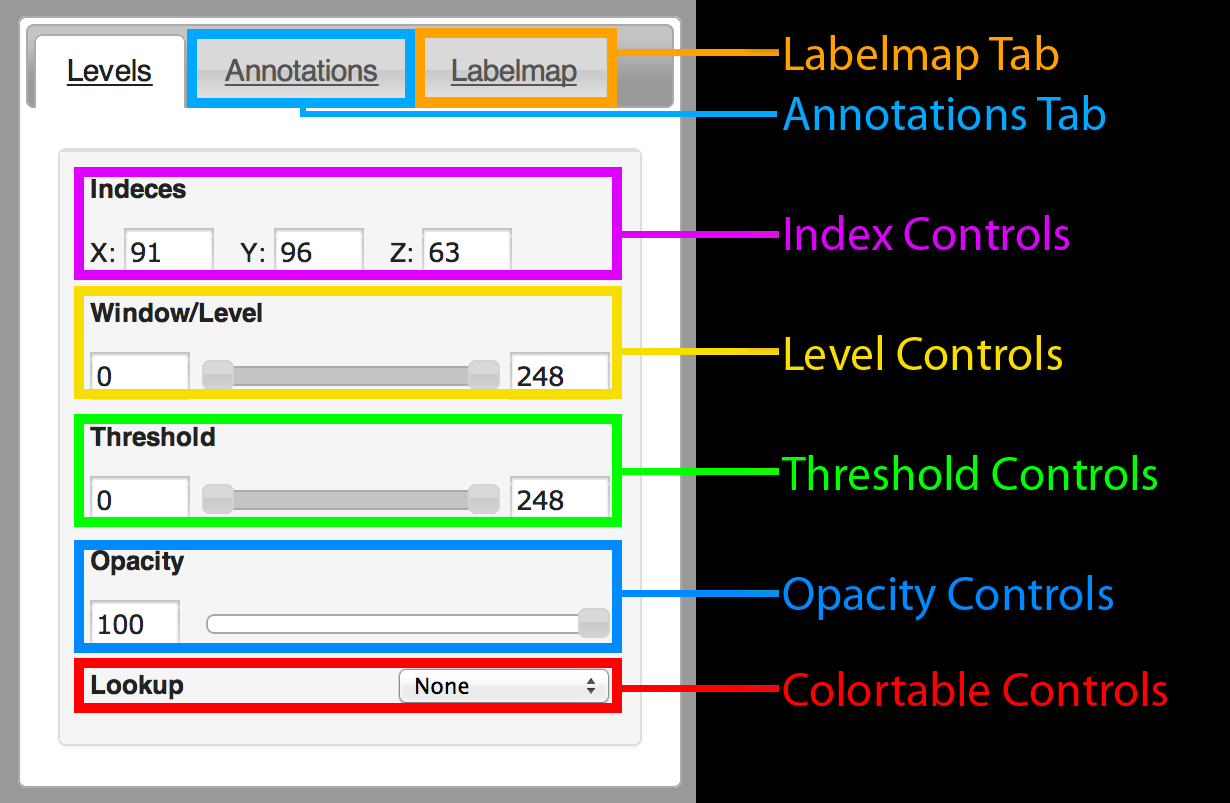
\includegraphics[width=90mm]{graphics/features_04.png}
\caption{Levels Tab Functionality}
\label{fig:UIdesign1}
\end{figure}



\begin{figure}[ht!]
\centering
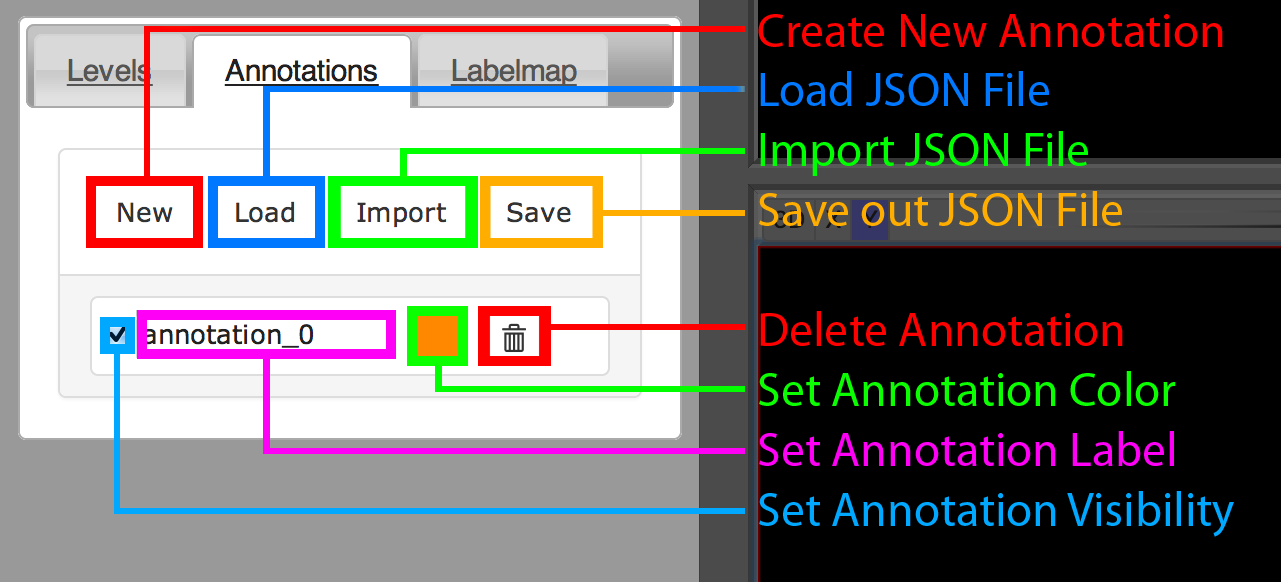
\includegraphics[width=90mm]{graphics/features_05.png}
\caption{Annotation Tab Functionality}
\label{fig:UIdesign1}
\end{figure}



\begin{figure}[ht!]
\centering
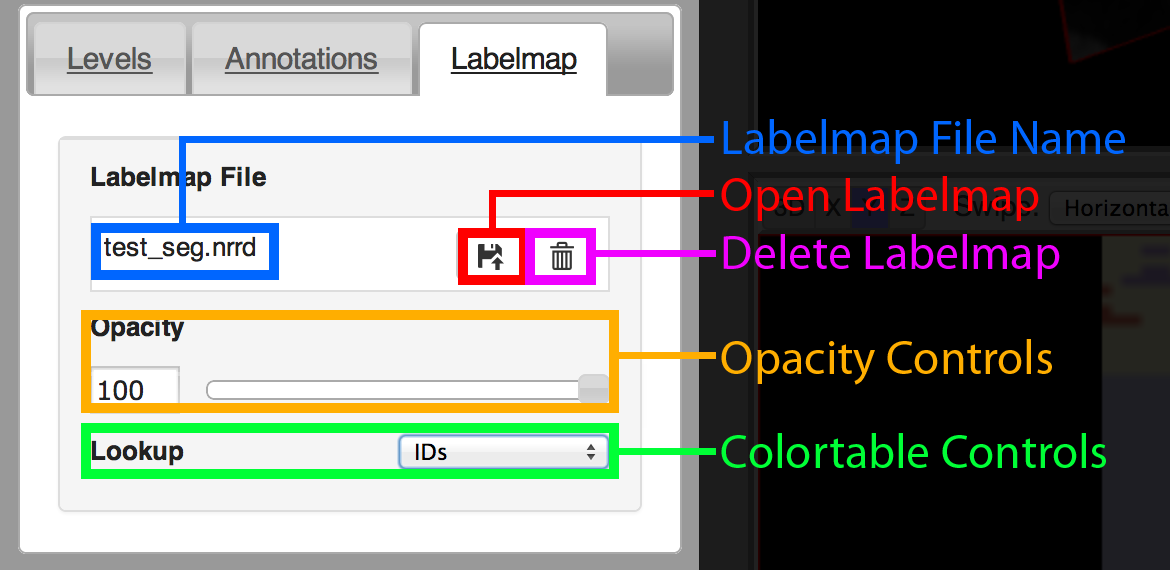
\includegraphics[width=90mm]{graphics/features_06.png}
\caption{Labelmap Tab Functionality}
\label{fig:UIdesign1}
\end{figure}


\subsubsection{Labelmaps}


\subsection{Development Strategy}

Generally program in modular fashion, tackle problems in a naive fashion first to test for any big problems. Once a certain prototype milestone had been achieved, some time spent refactoring based on insights learned. Arguable if  better planning would have been more time efficient.

\subsubsection{Meetings with Supervisor}

- supervisor seen as client
- meetings every 1 to 3 weeks
- notes taken, feature requests taken on board

\subsubsection{Coding Journal}

As the project grew more complex, I started writing a Coding Journal in which I would write down any relevant ideas or thoughts. Since working on one aspect usually took more time than thinking of ideas for other aspects, this proved quite valuable in recording them, organising them and going back over later to make sure I had not missed anything important.

\subsubsection{StackOverflow}

As I am sure is a regular occurence, checking StackOverflow for any problems proved invaluable. There are x posts on the topic of Backbone, JavaScript and Jquery, so it provided a vast resource for fixing problems. XTK is relatively small but still useful due to the occasional answer of the XTK authors themselves.






\subsection{Implementing Features}


\subsubsection{Creating the structure}

I started the project with one of the tutorial from the XTK website. Tutorial 13 had a very basic setup that was similar to what I intended for my project - a 4 view rendering of a data file. The tutorial has less than 100 lines of Code, with half of it used for specifying an inbuilt GUI. Since I wanted to create a custom GUI and generally have a much bigger codebase, first I need to ensure that I had a solid structure for my project. This is where Backbone and RequireJS came into play. Since I was not entirely familiar with either of them, it took a few days to get up to speed and try out a few tutorials to familiarise myself with their useage. It was overwhelming at first and I had to take a leap of faith that everything would out. After a few days I had managed to create a frame work that mimicked the tutorial, but was running in the confines of Backbone with proper views and managed dependencies through RequireJS.

Need to talk about MVC MVP


\subsubsection{Loading Volume Files}

The next step was to enable to loading of local volume files. This can be tricky with web browsers, as for security reasons file I/O is not a feature that is readily supported. However I had the SliceDrop code to look through. Basically copying the data into a local container did the trick. This is done with the HTML5 FileReader element, which allows for asynchronous file loading in various formats (text/buffer, etc).

Once I had this setup I came across one of the first bugs in XTK. When loading NRRD files, the volume would load and display, but it would be slightly offset. Testing this on a couple of Desktop solutions which worked fine let to the conclusion that it is a bug in the XTK library. 

Picture



\subsubsection{Layout of Program}

In terms of the layout of the components of ScanView, I had fairly accurate ideas. It needed to accomodate the 4 different views in viewing panels (one 3D Camera View and X, Y and Z Camera Views). I wanted to add some customisation options in terms of size of the viewer and choice of Camera View in each panel. Depending on whether it was a 3D or 2D Camera View, the Display Panel would have different options. 3D Camera View needed a toggle for Volumetric Rendering, 2D Camera View needed a toggle for Information Overlay.



\begin{figure}[ht!]
\centering
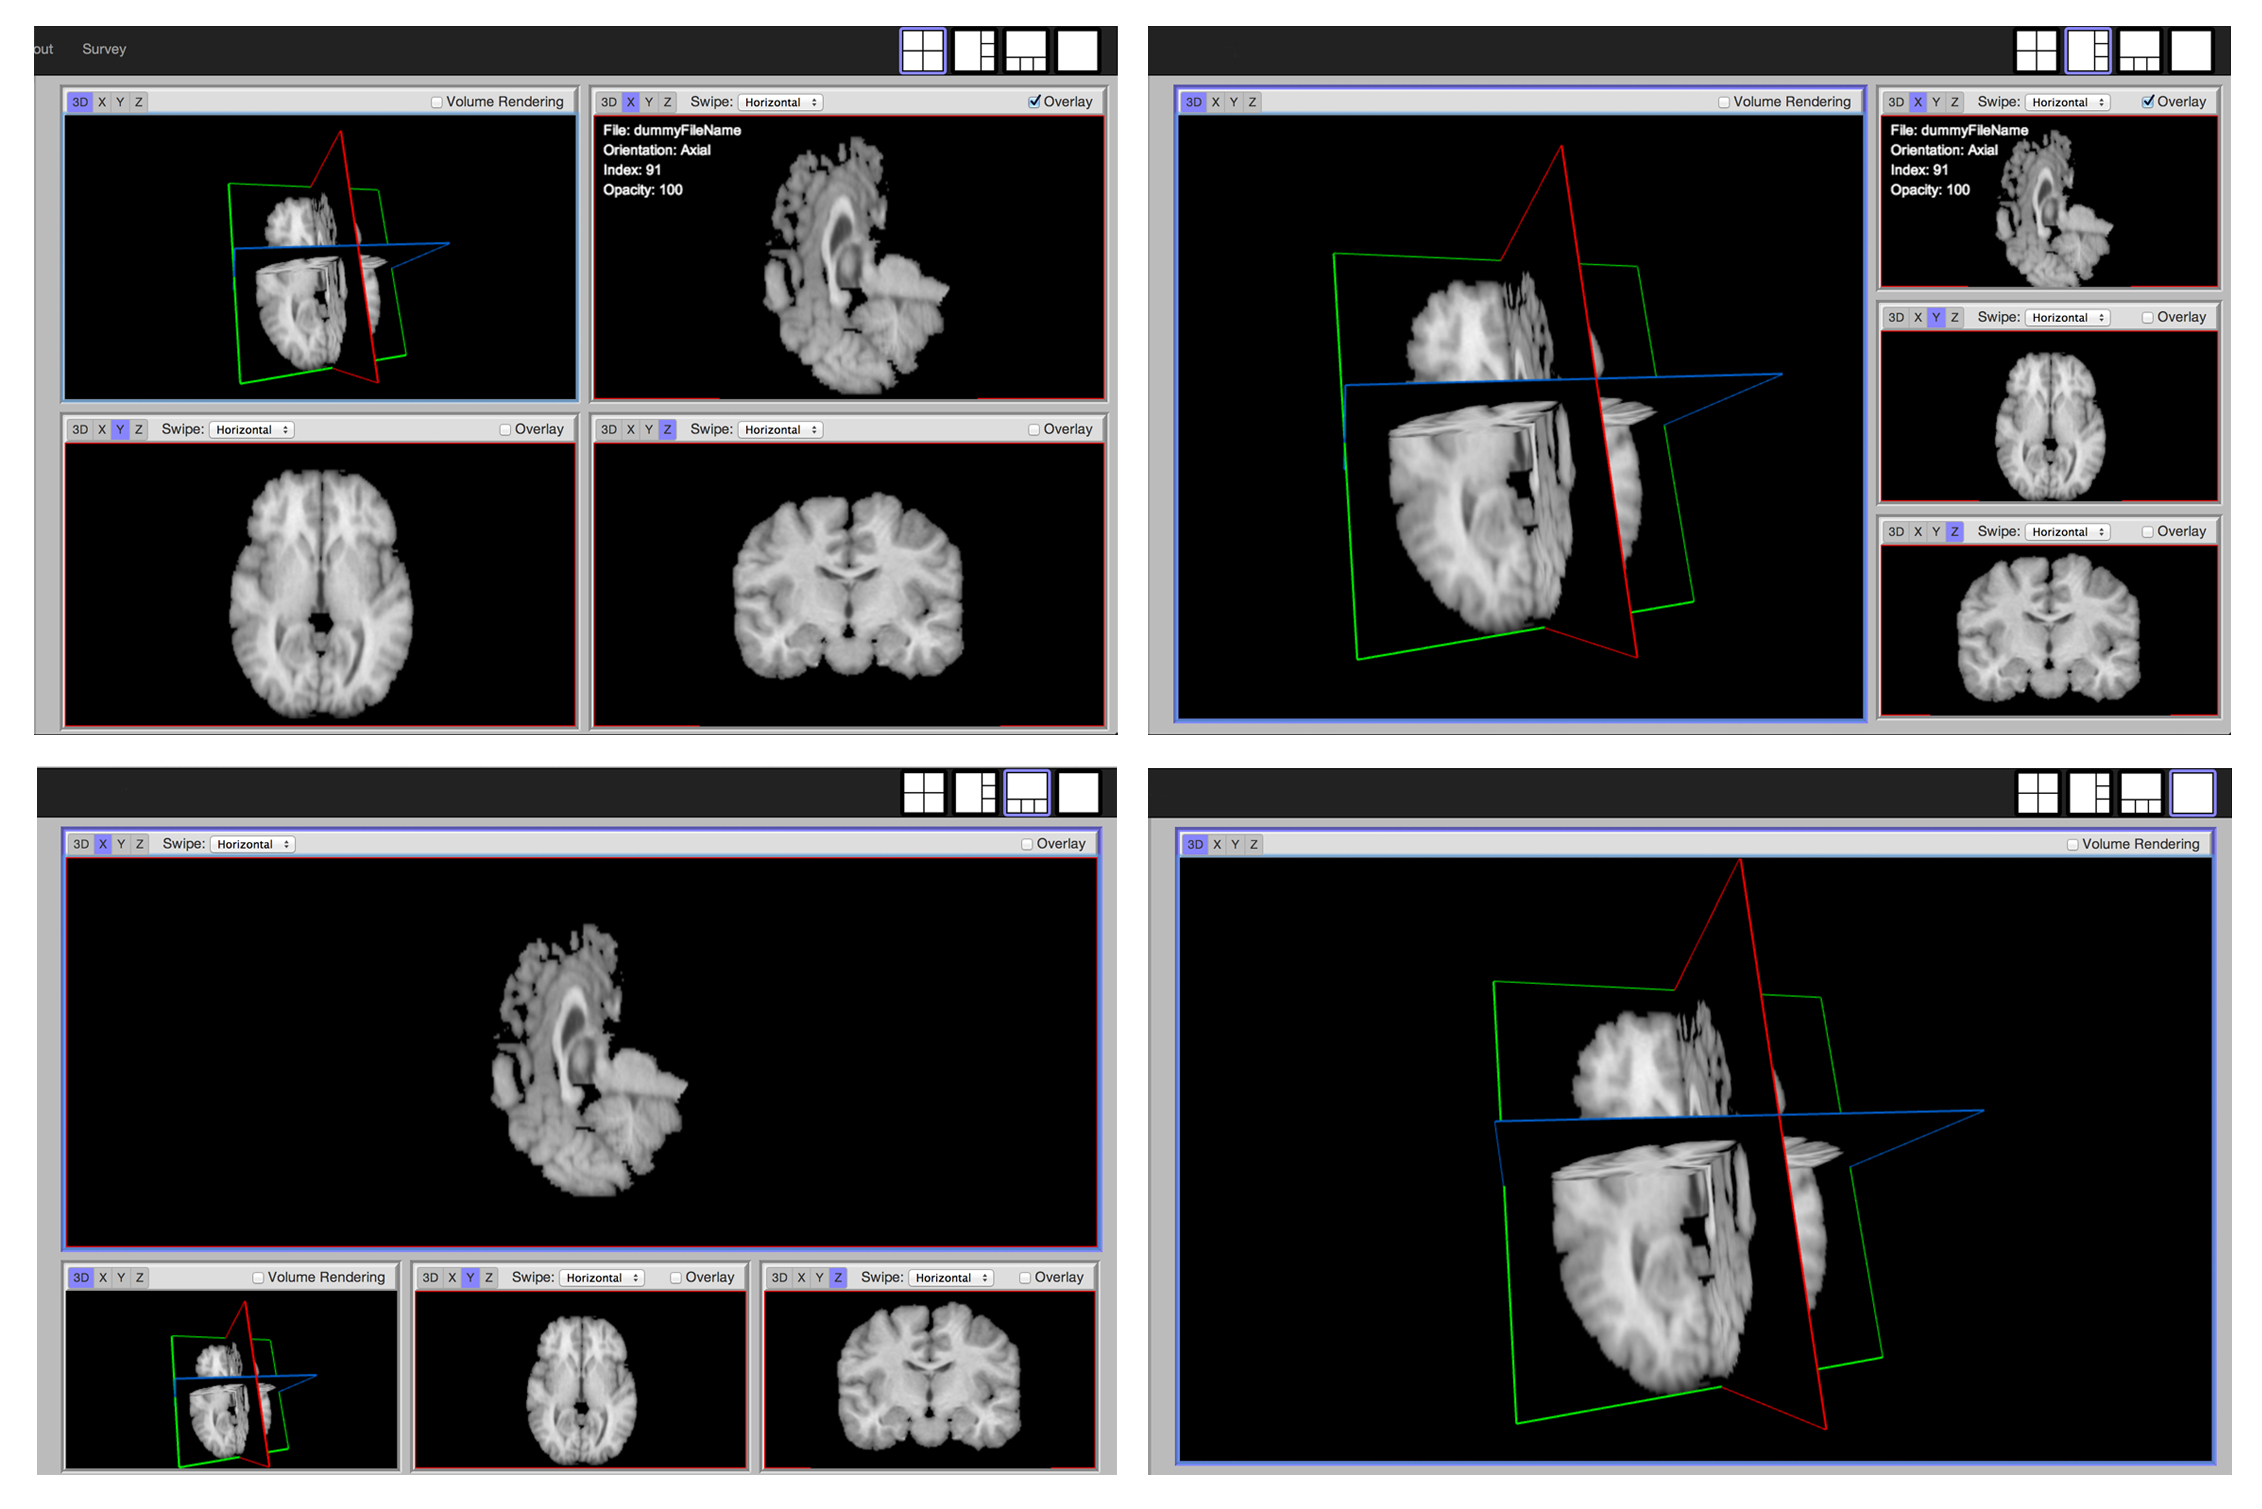
\includegraphics[width=170mm]{graphics/layouts_01.png}
\caption{Four Different Layout Options}
\label{fig:UIdesign1}
\end{figure}



For the different layouts I briefly investigated using interactive splitters, but found them to be not very easy or reliable to tie into the program. Instead I opted for 4 different static Layouts (See image below). This should give the user enough options to choose what his prefered layout. Implementing the logic behind these panels took a while to get right. Panels had to auto-resize everytime the layout was changed. Again this required some exposing of extra XTK attributes.




Coming up with a concept for the viewers... needed to have the distinct number of viewers.
Came up with concept of copying images from it.
Was trying to use it still as an API, did'nt realise that I would have to descend deep into the library at some point.



\subsubsection{Display Layer Management}

Layers

For each Layer, separate tools

Buffers


\subsubsection{Colortables}

The next feature I tackled was Colortables, with which to change the color output for a given volume. The XTL library does support Colortables, which ironically ended up costing me a week of coding time. XTK Colortables follow the same format as 3DSlicer's format and a Wikipedia site with which one can create custom Colortables exists online. The format is that each line is prefixed by an index, which will usually by the RGB value of the volume data. Each line is then mapped to a label and a set of RGBA values.

\begin{figure}[ht!]
\centering
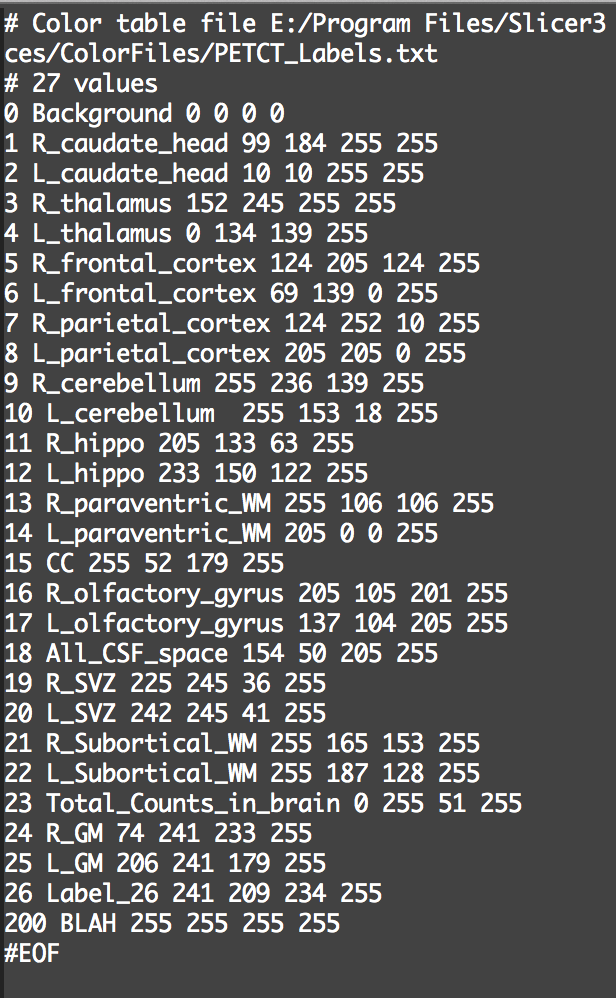
\includegraphics[width=70mm]{graphics/Colortable_01.png}
\caption{Example of a Colortable}
\label{fig:UIdesign1}
\end{figure}

XTK deals with Colortables in that the user has to load them as a .txt file when adding the Volume data and other input files. Thereby it is bundled up with the rest of the IO processes. Again, as with normal file loading, XTK is not designed for adding or modifying these kinds of files at runtime, so I had to add this functionality. This took a long time in that I had to trace the whole function flow of XTK when loading files. I proceeded with various steps, but would encounter problems at every stage, since I was forcing XTK do something that was not really inherent in its initial design. At a very basic level, colored displays (ie varying R, G and B channels) were not enabled for volumes by default, so I had to edit the code for that. On top of that, 2Drenderer and 3DRenderer deal with color and rendering quite differently. The 2D renderer does the rendering to screen space at a specific time per second. The 3D renderer uses a fragment shader (like in OpenGL) to assign color. Figuring all this out took a while, and after 7 days I had finally managed to get the whole process working. The only problem was that since I/O was involved, it would take quite a bit of time to update, so it was not entirely slick. Also, the way XTK loaded these colortables was by actually baking the colors into the slice texture. 


\begin{figure}[ht!]
\centering
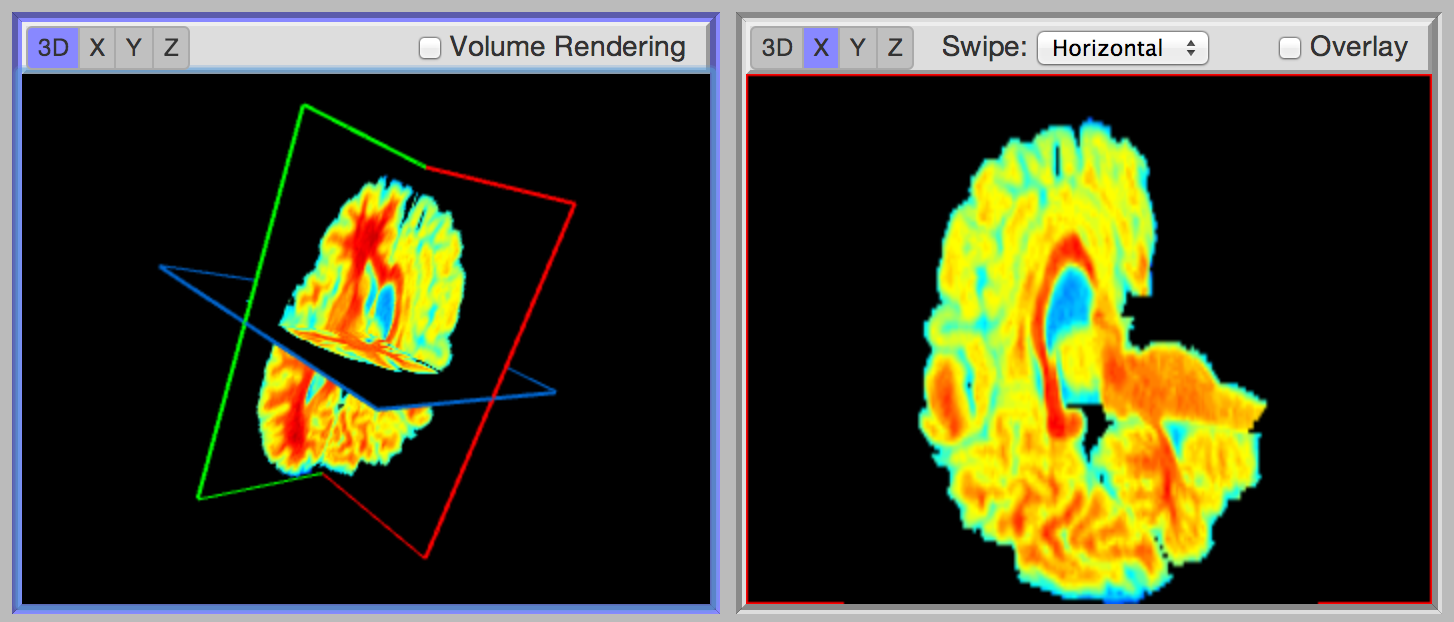
\includegraphics[width=170mm]{graphics/Colormap_01.png}
\caption{Brain Scan with 'Heatmap' Colortable applied in 3D and 2D View}
\label{fig:UIdesign1}
\end{figure}

\begin{figure}[ht!]
\centering
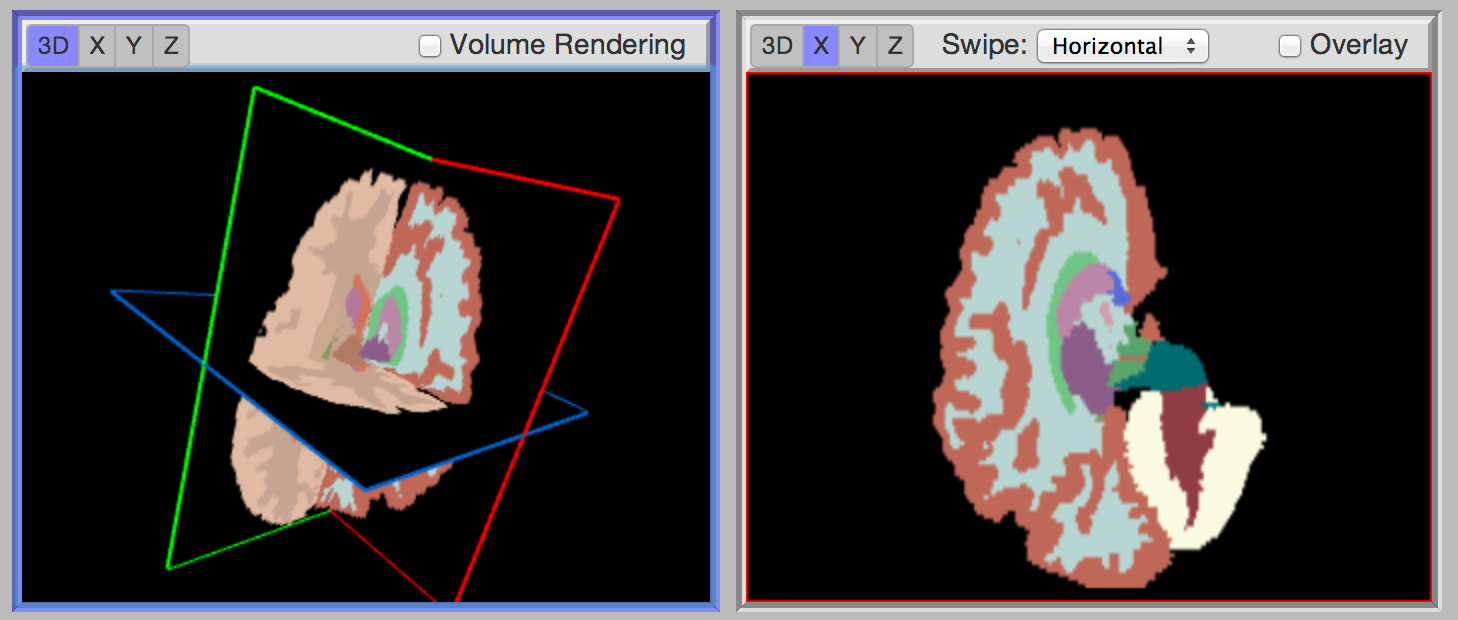
\includegraphics[width=170mm]{graphics/Colormap_02.png}
\caption{Brain Labelmap Scan with 'ID's' Colortable applied in 3D and 2D View}
\label{fig:UIdesign1}
\end{figure}


Having finished this feature so far, it occured to me that I could actually speed the whole process up by having some hardcoded colortables in the code, and using them as a array to look up colorvalues when rendering the actual pixel. This was much easier to implement, loads much quicker as it is more efficient in only manipulating color at a pixel level rather then changing the color values of the whole volume. In the end I chose this method as I prefered the faster feedback. It has the limitation that the user can not load his own colortable, but this is a feature that could be added in future. For the moment, there are three colortables provided. Firstly, the standard colortable maps rgbs values directly to the same value. Secondly, an ID map maps values to different RGB values, which is intended for use with labelmaps. Thirdly, a type of HEAT/JET map has been included which maps the original RGB values from BLUE to RED to mimic the behaviour of a heat map. This was advised by the project supervisor.


\subsubsection{Annotations}

\begin{figure}[ht!]
\centering
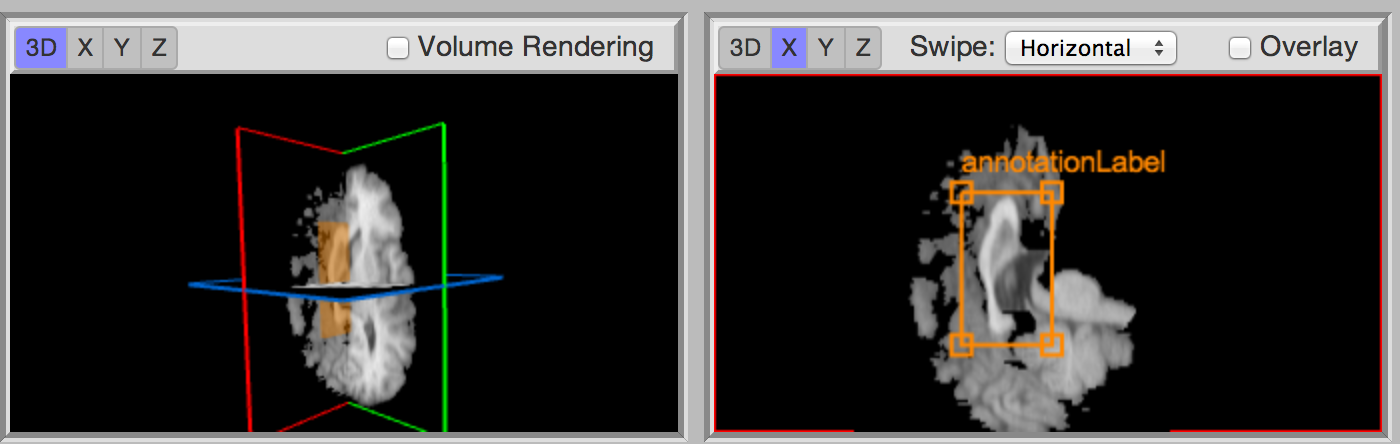
\includegraphics[width=170mm]{graphics/AnnotationFinal_01.png}
\caption{Annotation in 3D and 2D View}
\label{fig:UIdesign1}
\end{figure}

The Annotations feature was addded in the last month and I was aware of time pressure. That is why initital design decisions had to be made to reduce wasted time later in the process. I decided on implementing rectangular annotations first, since that would make calculations easier to manage. Annotations would be JavaScript objects with core members that were predefined (labelName, color, 3DPoints), and secondary attributes that would have to be computed on the fly (such as 2D Points for displaying on screen). Specifically, an annotation would be defined by 8 points in 3D Space. However to render it in a 2D View, 2D points had to be generated in screen space. I had intended the 2D points to be selectable in the Canvas View, so these 2D points should also be objects with custom attributes.

An initial UML diagram was desiged as below:

IMAGE




The final Annotation class contained quite a few more helper functions to help with the conversion from 3D to 2D space.


The next step was to chose a data format and design the workflow. Initial tests were done with XML but to be somewhat cumbersome since some parsing is required and in the program the XML structures would have to be converted to JavaScript objects. Therefore the much more intuitive JSON format was chosen, since this basically stores JavaScript objects in readable form, and can be loaded directly into the program without almost any conversion required. The JSON format was originally derived from JavaScript which explains its ease of use.

Probably the most involved work was to figure out the conversion of 3D points to 2D screen space. The 2D points would be calculated by each XTK renderer separately, since the different views required different 2D screen space points. An array of the 2D points would be stored in the Annotation class. These points would then be updated whenever the position of the 3D points of the Annotation changed. The XTK renderer class has a function that translates 2D screen coordinates to 3D slice index coordinates which was a good starting point. I chose a simplified version of this function and implemented a conversion function, which appeared to work fine. However some bugs were noticeable where all 2D points of an Annotation would sometimes jump by a pixel even when they were not being manipulated. I attributed this to some floating point or rounding errors, but could not track down where the errors were happening. Finally I had to admit that my simplified conversion function was not accurate enough, and I set out to reverse engineer the 2D to 3D conversion from the XTK library. This involved some inverse matrix multiplication, and in the end worked perfectly. These changes had to be made in the XTK renderer class.

In order for the user to manipulate the position of the Annotation points in screen space, I had to implement manipulatable corner points of the Annotation. This was made easy by the decision to have the 2D points. Initially I had contemplated creating a separate Manipulator class, but realised that this was superfluous and would just be repeating code. In the 2DPoint class I specified the position and width, so that in screen space I could make the 2DPoints appear wider for easier selection with the mouse. Some internal logic had to be added to the Annotation class, so that when the user changes the position of one 2DPoint, the neighboring points would also transform accordingly, since the shape had to always stay rectangular. I had to revise this is a couple of times, since in my first naive implementation, there would problems when the Annotation box would collapse so that all four 2D Points would be at the same screen space position. In the end I opted for limiting the size of the Annotation so that the points could never collapse to the same position.

Diagram of the annotation?


An important part of the Annotation Management was the feature to download Annotations as a JSON file. However again due to web browser security restrictions, there is no 'Save File As' feature as I had imagined. However after some research, a viable alternative was found in that it is possible to 'download' a file (even if the code is running locally). This was deemed sufficient for this project, even if it does not allow for specifying the file name directly. With more time, it would be possible to add a pop-up window just like a 'Save as' dialog that would then trigger the file download.

Saving files to JSON format was straight forward due to the before-mentioned natural overlap of JavaScript objects and JSON format. The saved files would only include the core information such labelName, color, 3D points and type.

To let the user specify a color for the Annotation, I needed to introduce a color picker. After some research, it became apparent that a host of color pickers were available online and it would be faster to use one of them than impement my own. I downloaded a couple of ColorPickers from the web, and deemed Blah's colorpicker to be better suited. It has a very basic interface that was deemed sufficient for chosing an Annotation color. Installing and implementing it into the project was also very straight forward.

Once I had implemented the code for creating and editing one Annotation, I created another layer system similar to main Display Layer management. Final tweaks to Annotation management include highlighting the Annotation Layer in the Layer View when hovering over or transforming one of the 2D Points.


\subsubsection{Labelmaps}

Adding Labelmaps proved to be relatively painless due to the time spent understanding the file loading process when implementing the colortables. The loader had to be forced to refresh when the labelmap was added on the fly. I restricted the program to only overlay one labelmap. I hooked up the opacity and colortables as for the Display Layers. I set the default colortable to chose the ID colortable preset, as that made more sense given the nature of labelmaps.

\begin{figure}[ht!]
\centering
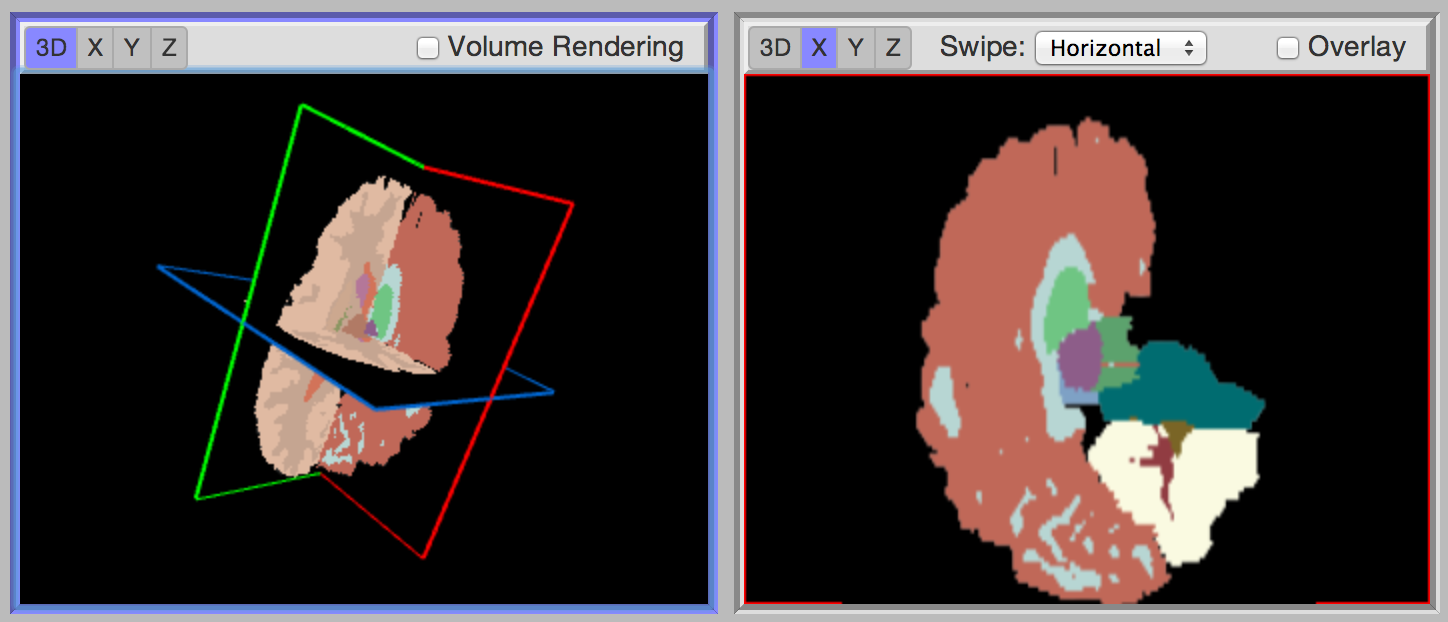
\includegraphics[width=170mm]{graphics/Labelmap_01.png}
\caption{Brain Scan with overlaid Labelmap}
\label{fig:UIdesign1}
\end{figure}




\subsection{Implementation Details}

\subsubsection{Version Control}

To keep track of my project, I used Git. This was an obvious choice since it has been the DOC-prefered version control system as well as XTK being hosted on Github which I had to fork. I managed my own project code in a separate Version Control from my XTK fork in order to not confuse the two. Github proved as per usual very useful and reliable in tracking down changes from earlier versions as well keep submodules up to date for the XTK library. 


\subsubsection{Browser Developer Environment}

Firefox being shit, not intuitive
Chrome being best
printing to console
Chrome providing Sources, like a debugger with line by line features

Throughout the project there were issues with different browsers behaving differently. For example the layout would look drastically different in Firefox compared to Chrome, sometimes for reasons that were hard to track down due to large amount of variables in play. It appeared as if the css float command behaved differently, and place items to a different rule set. At other times, mouse navigation would not work in Firefox, since somehow mouse clicks where registered differently from Chrome. During the project, I spent time trying to bring up browser compatibility for both in parallel, but in retrospect I probably should focused on Chrome, and then spent time making it work in Firefox and all other browsers, since they will also need custom work.



\subsubsection{XTK}

- bugs with XTK
- written with goog.closure library
	- uses minified code, uses a compiler
	- use the debug version
- extended the library
- exposing variables
- various event calls
- followed the XTK style guide
	- camelCase
	- underscores, public attributs

- explain the structure




\subsubsection{Backbone}



\subsubsection{RequireJS}

RequireJS proved invaluable for determining correct dependencies for loading JavaScript libraries.
As I am using more than a handful of libraries which are also dependent on one another, I needed the ability to ensure that they had loaded correctly. The issue is that the modules are loaded asynchronously, so a module that depends on a another module could easily load before the other (as opposed to in sequence loading from function programming). A good exampe for this is the tooltips that I implemented towards the final stages of the project. Both jQueryUI and twitter-bootstrap provide tooltips. In both cases they are initiated by the same function call, however they look quite distinctly different. I wanted to use the twitter-bootstrap tooltips as they seem more aesthetically pleasing. Without determining the load order with RequireJS, whenever I reloaded the software a different tooltip style would pop up, depending on which library loaded first. This kind of race condition is of course undesirable.
Another example is of course XTK itself which relies on JQuery and UnderscoreJS. RequireJS really was a life saver for these situations.






\subsubsection{JQueryUI}

Generally speaking, for any HTML page element, both the look and the functionality have to be considered, as implementing them can be quite complex. This is why a lot of libraries have been created that provide generalised elements such as buttons, file loaders and more complex UI elements. A few like JQueryUI and Twitter-Bootstrap have been become very popular and have been used in this project. They have the benefit of providing both the CSS style definitions as well as predefined JavaScript functionality for the elements. 

Some features from this library were utilised, such as the tab functionality for the 'Levels', 'Annotations' and 'Labelmaps' tabs. Also, the sliders for setting Brightness, Threshold and Opacity were taken from this library, as they provided a convenient solution both for the design and for the functionality.


\subsubsection{Twitter-Bootstrap}

This library was used to style the webpage consistently and to make use of their icons, buttons and tooltip functionality.

The library provides a host of useful icons and button presets, such as button groups which were used when grouping buttons close together like the 'Load' and 'Delete' button for each Display Layer. This added a more sophisticated look to the software without the need for individual styling of buttons by writing custom CSS classes.

Adding the tooltips proved more involved than initially thought. For dynamically added HTML elements such as the Display Layers, custom tooltip options would have to be used and set in order to make them work correctly. So instead of having a general purpose solution, custom settings had to be set for each tooltip. Also, since Twitter-Bootstrap and JqueryUI both provide tooltips that called by the same initialisation function, sometimes errors would appear in the browser console, stating that a conflict had been caused. Fortunatly, JQueryUI allows for downloading a custom build where the tooltip feature has been disabled.

Furthermore, creating modal warning screens when the user attempts to load a file with the wrong extension was made very easy with Twitter-Bootraps modal screen. Again, styling this manually and creating the logic behind it would have been very time consuming.

Twitter-Bootstrap supplies a host of interactive UI elements such as buttons, tooltips, pop up windows, tabs, navigation bars, progress bars and more. It is a widely used library - in June 2014 it was the No.1 project on GitHub with 69,000+ stars and 25,000+ forks (Wiki).


Picture



All things considered, this libary proved to be very useful and saved a lot of time.




\subsubsection{Google Analytics}

Google Analytics is a tool by Google that provides detailed information of count, frequency and location of website usage. I installed to get a clear picture of how many people would be using the website. I have used Google Analytics in the past and have been impressed by the comprehensive overview it provides. On top the expected visitor numbers, locations and duration, it provides percentage displays and other useful information.

Add diagrams if useful.





\subsubsection{User Experience}

Some effort was put into making the software intuitive for users to use.
This included the somewhat mundane disabling of all input and buttons when no appropriate medical imaging file had been loaded yet. Furthermore, pop up warning windows were introduced to warn a user if the wrong kind of file was being loaded. Tooltips were added to almost every button to help the user understand the intended functionality of each.

All navigation and traversal was placed on mouse controls. The guidelines from the book helped inform the controls in that radiologist prefer to have as simple controls as possible since their work can consist of dealing with vast quantities of these kind of files, so any intricate control input method would soon get tiresome.














\section{Results and Evaluation}

In order to evaluate the software, two components were chosen. The first was to test one of the main claims of this project, namely that the website runs on a variety of computer setups, thereby freeing the user of having to use a specific desktop tool for a specific platform. Secondly, the software has been deployed on the Internet and has been sent to a number of users for evaluation via a survey. Finally the software will be evaluated against the aims set forth at the beginning of the project.
Evaluation of main client?


\subsection{Protocol Testing across different platforms}

In order to judge whether the software fulfils its purpose of running on a variety of operating systems and web browsers, a number of protocols were tested across a range of computer setups. It was tested on the four most commonly used web browsers and on Windows, OSX Mavericks, Linux (Ubuntu) and Android. Additionally a test was run for the Apple I-Pad. The protocols were designed to mimic what a typcial user would do with the software as well as to get a comprehensive coverage of all the features.


\subsubsection{Protocols}

\subsubsection*{Protocol 1 - Basic Viewing of Volume File }

- Create a Display Layer\\
- Load a medical image data file (.nii)\\
- Test navigation - pan/zoom/rotate/traverse\\
- Test window levels\\
- Test threshold\\
- Test changing color lookup\\
- Test the different layouts\\
- Test switching Camera Views

\subsubsection*{Protocol 2 - Creation of Annotation }

- Create a Display Layer\\
- Load a medical image data file (.nii)\\
- Create a new annotation\\
- Change annotation label\\
- Change annotation color\\
- Change annotation vertex points

\subsubsection*{Protocol 3 - Loading and Saving of Annotations }

- Create Display Layer\\
- Load a medical image data file (.nii)\\
- Load/Import annotation JSON file\\
- Change annotation color\\
- Change annotation vertex points\\
- Save out annotation


\subsubsection*{Protocol 4 - Labelmaps }

- Create Display Layer\\
- Load a medical image data file (.nii)\\
- Load a labelmap file\\
- Set opacity of labelmap file\\
- Change color lookup for labelmap

\subsubsection*{Protocol 5 - Display Layer Management }

- Create Display Layer\\
- Load a medical image data file (.nii)\\
- Create a second Display Layer\\
- Load a second medical image data file (.nii)\\
- Toggle between buffers\\
- Test opacity slider\\
- Test horizontal swipe\\
- Delete First Display Layer\\
- Test basic viewing\\
- Delete Second Display Layer




\subsubsection{Testing Environments}


\subsubsection*{OSX Mavericks}

For OSX the website was tested on the latest OSX Mavericks Operating System, installed on a Mac Book Pro. All protocols were run successfully for both Chrome and Firefox.\\

\noindent Hardware:\\
- Model Name:	MacBook Pro\\
- Processor Name:	Intel Core i7\\
- Processor Speed:	2.3 GHz\\
- Number of Processors:	1\\
- Total Number of Cores:	4\\
- L2 Cache (per Core):	256 KB\\
- L3 Cache:	6 MB\\
- Memory:	16 GB\\


\noindent Operating System:\\
- OS X 10.9.4\\

\noindent Browsers Tested:\\
- Chrome Version 36.0.1985.143\\
- Firefox Version 31.0\\
- Internet Explorer - Not available
- Safari Version 7.0.6 (9537.78.2)\\

\subsubsection*{Windows 7}

For Windows the website was tested on Windows 7, running on a virtual machine on a Mac Book Pro with the same specification as the previous section.\\

\noindent Hardware:\\
- Running via VMware Fusion on same MacBook Pro as used for testing OSX Mavericks\\

\noindent Operating System:\\
- Windows 7 Professional N Service Pack 1\\

\noindent Browsers Tested:\\
- Chrome Version 36.0.1985.143\\
- Firefox Version 31.0\\
- Internet Explorer 8.0.7601.17514\\
- Safari Version 5.1.7\\


\subsubsection*{Linux Ubuntu}

For Windows the website was tested on Windows 7, running on a virtual machine on a Mac Book Pro with the same specification as the previous section.\\

\noindent Hardware:\\
- Running via VMware Fusion on MacBook Pro as used for testing OSX Mavericks and Windows 7\\

\noindent Operating System:\\
- Ubuntu 14.04 LTS\\

\noindent Browsers Tested:\\
- Chrome Version 36.0.1985.143\\
- Firefox Version 28.0\\
- Internet Explorer - Not available\\
- Safari Version - Not available


\subsubsection*{IOS}

For IOS the website was tested on a Ipad Air. It was fairly clear that this would not work well, since IOS is a closed system that does not allow a free file structure as required by this software. However it was still checked to get a wider coverage of platforms.\\

\noindent Hardware:\\
- Ipad Air\\

\noindent Operating System:\\
- IOS V.XX\\

\noindent Browsers Tested:\\
- Safari Version XX



\subsubsection{Protocol Results}

\subsubsection*{OSX Mavericks}

All protocols were run successfully for both Chrome and Firefox. When using Safari, they were issues with loading Annotations and Navigation control. This should be fixable by simply investing more time into the project.\\


\begin{center}
  \begin{tabular}{ | l || l | l | l | l |}
    \hline
    Protocol & Chrome & Firefox & Internet Explorer & Safari \\ \hline \hline
    1 & Yes & Yes  & - & No   \\ \hline
    2 & Yes & No & - & Yes \\ \hline
    3 & Yes & No & - & Yes  \\ \hline
    4 & Yes & No & - & Yes  \\ \hline
    5 & Yes & No & - & Yes  \\
    \hline
  \end{tabular}
\end{center}

\subsubsection*{Windows 7}

All protocols were run successfully for both Chrome and Firefox. There were lots of issues with Internet Explorer, which was expected since it is renown for being difficult to code for and not following conventions of the other browers. Safari issues were also abound.

\begin{center}

  \begin{tabular}{ | l || l | l | l | l |}
    \hline
    Protocol & Chrome & Firefox & Internet Explorer & Safari \\ \hline \hline
    1 & Yes & Yes  & No  & - \\ \hline
    2 & Yes & No & Yes & - \\ \hline
    3 & Yes & No & Yes & - \\ \hline
    4 & Yes & No & Yes & - \\ \hline
    5 & Yes & No & Yes & - \\
    \hline
  \end{tabular}

\end{center}

\subsubsection*{Linux Ubuntu}

For Linux the website was tested on Ubuntu on a computer in the Department of Computing at Imperial College. Again, Chrome and Firefox performed well. Safari and Chrome were unfortunately not available for testing.

\begin{center}

  \begin{tabular}{ | l || l | l | l | l |}
    \hline
    Protocol & Chrome & Firefox & Internet Explorer & Safari \\ \hline \hline
    1 & Yes & Yes  & -  & - \\ \hline
    2 & Yes & No & - & - \\ \hline
    3 & Yes & No & - & - \\ \hline
    4 & Yes & No & - & - \\ \hline
    5 & Yes & No & - & - \\
    \hline
  \end{tabular}

\end{center}


\subsubsection*{IOS}

As expected, most functionality did not work on the Ipad. The display layer management worked fine, however the user is not able to load a file, since the default file opening only allows opening photos. However, it would be possible to circumvent this by implementing a solution that uses a file loading app, such as Dropbox. The Driopbox API seems to allow for this, so it could be possible given extra time.

\begin{center}

  \begin{tabular}{ | l || l | l | l | l |}
    \hline
    Protocol & Chrome & Firefox & Internet Explorer & Safari \\ \hline \hline
    1 & - & -  & -  & No \\ \hline
    2 & - & - & - & No \\ \hline
    3 & - & - & - & No \\ \hline
    4 & - & - & - & No \\ \hline
    5 & - & - & - & No \\
    \hline
  \end{tabular}

\end{center}


\subsection{CPU performance}

It has to be noted that the CPU usage is higher in ScanView than the original XTK apps. This is large part due to the design choice of copying the renders from the XTK renderers as discussed in the implementation. This accounts for the majority of the computational overhead. CPU comparisons were run in the Chrome - OSX environment and look as follows.
In order to improve performance, RequestAnimationFrame was used. Need some more text explaing what this does.



\subsection{Usage and User Feedback}

In order for users to be able to evaluate the product, some effort had to be put in to deploy the software to the web. This went smoothly, as it had been desiged as a live webpage from the beginning. So I added a page with some sample data for the user to download, tutorials resembling the protocols above together with screen capture videos. Furthermore an 'About' page was added which explained the main features of the program as well crediting various libraries and plug-ins that were used. Finally, an online survey by Survey Monkey was introduced to allow for convenient feedback by the user.

Ideally the website would be online for a longer time to get a more complete picture in terms of usage.
Analyse the usage reports from Google Analytics if appropriate.

A frustrating side effect of the survey
was not being able to get back individually and not being able to interface personally in order to fully interact and follow the users. However this is consequence of the limited time provided for the project, and it just took so long to get all the features implemented. In future, this time should be budgeted for in advance, so that a period of beta testing can happen on various platforms.

\subsubsection{Criticisms}


\subsubsection{Feature Requests}


\subsubsection{Outstanding Feedback}

I sent a link to the software to the XTK developers in order to get their feedback, but at this point in time have not heard back from them.



\subsection{Review of Features}


Discuss completeness of features. Satisfies most like others.
Compare it to SliceDrop. Compare it to Desktop Software!
Need to do a bit more research of



\begin{center}

  \begin{tabular}{ | l | l | l |}
    \hline
    Feature & ScanView & SliceDrop \\ \hline \hline

Loading NII file & Yes & Yes \\ \hline
Loading Other file formats & No & Yes \\ \hline
Loading multiple files in one session & Yes & No \\ \hline
Volumetric rendering & Yes & Yes \\ \hline
Volumetric and 2D rendering overlaid & No & Yes \\ \hline
Comparing several files to each other & Yes & No \\ \hline
Annotations & Yes & No \\ \hline
Loading of custom colortables & No & Yes \\ \hline
Loading predefined colortables & Yes & No \\ \hline
Saving of Data & No & Yes \\ \hline
Online File Sharing & No & No* \\ \hline

  \end{tabular}\\


*Not currently available but being worked on


\end{center}







\section{Conclusions}

In terms of the initial purpose of this project to investigate whether it is possible to create a feature rich medical image viewer which works in a web browser, the course of the project seems to suggest that it is indeed possible given current Web standards with HTML5 Canvas Element and the WebGL standard becoming common-place. The XTK library forms a solid base for adding more features such as in this project. In order to add more complexity, a method was chosen which requires more CPU power than the normal XTK library.

In terms of creating a function piece of software, more time would have been benificial to iron out bugs. Also it would have been great to have a bigger pool of sample data to work from, as there seem to certain files that do not open with this software. Given the limited time frame and man power, ScanView does not match the feature richness and performance of high-end software solutions. However this is not a limitation based on the technical possibilities of web browser technology, so should be feasible. One issue might be the complexity of scale, as software solutions such as BrainSomething are 400MB. That would be too much to load in a web browser, so a more complex memory management would be required.




\section{Future Work}

\subsection{Limitations}


\subsection{Known Problems and Bugs}

- High CPU usage
- not able to open certain .nii files, due to XTK library though
- more complex file error management
- ColorPopup not at the right position when at bottom


\subsection{Future Improvements}

online file sharing (ala DropBox), could make it workable on Ipad!
need to make it work on different resolution screens

numerous improvements:
- add paint tools
- add support for 4D data sets
- tweak performance
- UX improvements such as smart sliders
- technical improvements such as specify filtering
- splitters for the panes











\newpage

\begin{thebibliography}{1}

\end{thebibliography}

\newpage

\section{Appendix}



- Talk about DRY, UML Style Diagrams!




\end{document}
